\documentclass[english,12pt]{article}

\usepackage[english]{babel}
\usepackage[utf8]{inputenc}
\usepackage[T1]{fontenc}
\usepackage{hyperref}
\usepackage{siunitx}
\usepackage{graphicx}

\usepackage[hmargin=1in,vmargin=1in]{geometry}


\begin{document}

\begin{center}

\thispagestyle{empty}

$ $

\vspace{250pt}

\begin{bfseries}

{\Large Object Recognition and Path Smoothing Robot, Phase 3}

{\Huge Test Plan}

%{\Large $\langle$application and version to be tested$\rangle$}%

\end{bfseries}

\vspace{180pt}

University of Washington Tacoma, School of Engineering and Technology

%TIE-21204 Ohjelmistojen testaus%

\vspace{12pt}

Authors: 

Ammon Dodson \href{mailto:ammon0@uw.edu}{ammon0@uw.edu} 

Alex Marlow \href{mailto:alexmarlow117@gmail.com}{alexmarlow117@gmail.com} 

Jake McKenzie \href{mailto:jake314@uw.edu}{jake314@uw.edu}

Distribution: Matthew Tolentino

Document state: draft

Modified: \today

\end{center}

\newpage


\tableofcontents

\newpage


\section{Revision History}

\begin{itemize}
	\item v0.1: In this version of the testplan we defined the  
    scope of the problem with the introduction, test items and 
    approach.
    \item v0.2: In this version of the testplan we defined the  
    test items, schedule and approach.
    \item v0.3: In this version of the testplan we updated 
    the hardware, software, and system test items with 
    tables and test descriptions. 
\end{itemize}


\section{Introduction}
\subsection{Purpose}
This test plan describes the testing approach and overall 
framework that will drive the testing of the ORPS-Robot 
version 0.1 – The Object Recognition and Path Smoothing 
robot. The document introduces:
\begin{itemize}
	\item[] Test Strategy: These are the rules the test will e based on including 
    the givens of the project (e.g.: start / end dates, objectives, assumptions); 
    description of the process to set up a valid test (e.g.: entry / exit criteria, 
    creation of test cases, specific tasks to perform and scheduling)
	\item[] Execution Strategy: describes how the test will be performed 
    and process to identify and report problems, and to fix and implement 
    fixes.
    \item[] Test Management: process to handle the logistics of the test 
    and all the events that come up during execution (e.g.: communications, 
    escalation procedures and risk mitigation)
\end{itemize}
\subsection{Project Overview}
The ORPS-Robot will be a platform for validating the research of Michael McCourt 
and a scheme for exploring object recognition via OpenCV with Robot Operating System, 
which is a powerful framework for writing robot software. There will be a demonstration 
of Simultaneous Localization and Mapping (SLAM). Together this will demonstrate a ``finder
robot'' with applications in search and rescue and threat detection. Additionally there 
will be beacon triangulation and/or GPS to fuse additional location information into the 
SLAM or finder functionality.
\subsection{Criticality}
Failures can rarely be forecasted. But what we can do is establish a hierarchy of 
criticality to ensure that we are keeping up with the most important test and using 
other tests as needed. Ordering what we need to do by priority is important as the scope 
of the project grows. The reason for the priority emphasis is that it is by far 
the most efficient way of working, in terms of creating reliable products and reducing 
the overall cost of the project. For instance using the wrong battery on the ORPS-Robot 
would likely ruin at least the Raspberry Pi or OpenCR, along with other mission critical 
components. This is not only a likely outcome if special care is not paid but we have seen it 
happen with prior groups in previous projects in this program. For this reason a heavy emphasis 
will be paid on this scheme.
\centerline{
\includegraphics[width = \textwidth]{crit.jpg}}
\begin{itemize}
    \item[S1.] Secondary Service - These involve services that are only checked when a component 
    fails. Use see in many applications test conditions can take longer to create than others. 
    This is the sort of service that happens ala cart and may be indistinguishable from the actual 
    build and design process in spots. These are components that we should likely assume work until 
    they don't.
    \item[S2.] Critical or Primary Service - Most component tests, both software and hardware, 
    fall under this category. Some but not all integration test that fall under interaction of 
    components (system test items) will likely fall under this category. These are services that 
    if they fail, will not mean the end of the project, but are extremely critical components 
    and should be worried about early and often.
    \item[S3.] Mission Critical Service - Most acceptance tests will fall under this category, this 
    means systems test items critical to Dr. McCourt’s research and of our object recognition 
    portion. A lot of integration testing will follow under this category. These are services 
    that if they fail, then the project has serious issues that need to be resolved.
\end{itemize}
\subsection{Audience}
Collaborative robotics software development for research in control systems 
for path smoothing. Collaboration in academic research is usually thought to mean 
equal partnership between two academic faculty members who are pursuing mutually 
interesting and beneficial research. In our case we are creating a platform which 
will serve Dr. McCourt's research where deep understanding of the control system in 
place is not require on our part and a deep understanding of the robot are not 
require on the part of Dr. McCourt.\\\\
Creating truly, robust, general-purpose robot software is hard. As 
undergraduates using the robot operating system framework allows us to encompass 
solving robotics problems in real-world variations in complex tasks and 
environments that no single individual, laboratory, or institution could 
hole to create completely on their own from scratch. The audience for this 
device is us, as it serves our education.\\\\
Applications in path smoothing and object recognition used in 
ORPS-Robot project are heavily used in semi-autonomous and autonomous 
vehicles. The knowledge gained in applying these skills in the ROS ecosystem 
should serve us to gaining a greater knowledge of the systems and 
practices of both control systems and object recognition.
\section{Test Items}
\subsection{Hardware Test Items}
Hardware testing is the exercising of a piece of hardware. Which often times involves the 
ability to take measurements along the way with a generated record of the whole process. Testing 
must be cataloged and recorded. While this is mostly a software project hardware testing for the 
ORPS-Robot, should and will be split into four key modes:\\
\begin{itemize}
\item[M1.] Electrical Testing: This is one type of test, unlike software testing, that 
poses a verifiable risk of physical danger to the test and system under test. Even a system that 
is not powered can have potentially have deadly electrical charges stored in capacitors and batteries. 
For the purposes of ORPS-Robot most electrical tests will be in the form of connectivity testing 
and the testing of the battery on the robot itself. 
\item[M2.] Environmental Testing: This is the testing of the device with things as they are, 
not how we would like them to be. This is to see how a system responds to various types of insults, 
justifiable hurdles and taxing conditions. For this project we will be testing how the ORPS-robot 
responds to various stimuli including windows, people, interferences over the Wi-Fi, LiDAR and 
ultrasonic signals and other stimuli yet to be discovered. The system must be tested and verified to deal 
with such stimuli.
\item[M3.] Mechanical Testing: Anything that can bend, click, flex, is in any way subject to opposing 
forces, latch, open and close, plug and unplug, press and depress, rotate, or switch and toggle, might 
eventually fail and will be subject to strains and wear. For this project the main mechanical component 
that must be dealt with are the DYNAMIXEL actuator system and wheels and LiDAR. 
\item[M4.] Integrated Software: Poor maintenance of the BIOS and firmware on a system can ripple through to 
affect both hardware and software, causing reliability issues for the system under test. Good software principles, 
for this reason, make good hardware and for this reason this goes in the hardware testing.  For the ORPS-robot 
our BIOS and firmware make up a huge aspect of the project itself. Much of that is up to us to control and tune, 
not some third party. For this reason, it is identified that this is a major key area of the project. This will 
also include the most fundamental of hardware tests: subsystem sanity tests, which are no more than tests that 
run whenever a system reboots or power ups. These must be employed on the ORPS-Robot to ensure a first line of 
defense in isolating hardware issues.
\end{itemize}
The ideas for these modes were borrowed heavily from Managing the Testing Process by Rex Black 3rd Edition, 
Appendix A: Hardware Testing Fundamentals. 
\begin{itemize}
\item[H1.] \ang{360} LiDAR for SLAM \& Navigation
\item[H2.] Raspberry Pi 3 Model B
\item[H3.] 32-bit ARM Cortex-M7 OpenCR
\item[H3.] DYNAMIXEL actuator system and wheels
\item[H4.] Li-Po Battery 11.1V 1,800mAh 
\item[H5.] Xbox 360 Controller 
\item[H6.] Marvelmind Sensors
\end{itemize}
Connectivity on the Raspberry Pi 3 Model B and 
\href{http://emanual.robotis.com/docs/en/parts/controller/opencr10/}{\textit{32-bit ARM Cortex-M7 OpenCR}} 
must be completed regularly. The Li-Po Battery 11.1V 1,800mAh will need to have its voltage checked to 
regularly. To assist in this process only batteries that match our desired voltage and amperage will be 
used, as they will have some sort of marking (coloured tape) to distinguish from other batteries that may 
exist in the lab. The DYNAMIXEL actuator system and wheels will need some sort of test. We do not know what 
that looks like at this time but that falls into the category of mechanical testing. The integrated software 
will be the test most frequently ran, as this is a test ran whenever the device is booted up. If problems arise, 
that puts a halt on the entire project so dealing witch such issues should have a methodological approach to stamping 
them out. 
\subsection{Software Test Items}
At this point in the process we do not know what the overall architecture of the software will 
look like but we can have a general plan of attack for writing software tests using rostest. According 
to Paul Ammann's Introduction to Software Testing, there are five levels of software testing: \\
\begin{itemize}
    \item[Level 0] There is no difference between testing and debugging.
    \item[Level 1] The purpose of testing is to show correctness.
    \item[Level 2] The purpose of testing is to show that software does not work.
    \item[Level 3] The purpose of testing is not to prove anything specific, 
    but to reduce the risk of using the software.
    \item[Level 4] Testing is a mental discipline that helps all IT professionals 
    develop higher-quality software.
\end{itemize}
For our purposes levels 0 through 2 will be used heavily in this process while level 3 and 4 will 
only be used when needed. To accomplish the task in level 0 we will be making heavy use of first 
GDB (C debugger) and PDB (Python debugger) along with Valgrind. Levels 1 and 2 will be tackled, 
hopefully, by making heavy use of \href{http://wiki.ros.org/rostest}{\textit{rostest}} which is an 
extension of roslaunch that enables roslaunch files to be used as text fixtures. Due to complex 
behaviors involved in this project we need to write tests and move on from functionality. When we 
introduce new functionality to the to ORPS-robot it will need to pass the old tests we wrote for it. 
if everything is functioning properly there should be no need to re-write our old tests. This will 
likely only be done with software strict aspects of the project as hardware is subject to change as 
the implementation changes over time. These tests, at least of the framing of this writing, will be 
to test the linking of different scripts and files written in the overall project. 
\subsection{System Test Items}
For the \ang{360} LiDAR for SLAM \& Navigation we will need to consult three separate 
resources for testing the LiDAR. The first will be a github wiki page entitled 
``\href{https://github.com/robopeak/rplidar_ros/wiki/How-to-use-rplidar}{How to use rplidar}'' 
which is just a walk-through of how to get rplidar ros package working. While this just gives 
a short introduction to rplidar, a more up to date tutorial on quickly getting rplidar up and 
running can be found on Service Engineering Research Area website under 
``\href{https://blog.zhaw.ch/icclab/rplidar/}{From unboxing RPLIDAR to running in ROS in 10 
minutes flat}''. The first goal with LiDAR appears to be establishing the range of the device 
as this what determines the quality of the information used in navigation. Given more time 
there will also involve be static and dynamic tests based on scanning calibration, 
speed of the LiDAR, vehicle speed, laser position feedback. Further testing will involve the use 
of a tutorial on husarion.com entitled \\\\
``\href{https://husarion.com/tutorials/ros-tutorials/6-slam-navigation/}{SLAM navigation}''. 
According to the Bachelor's Thesis of Felix Feik from Technical University of Munich,
the most difficult factor in indoor mapping using LiDAR is that the laser sensor always has 
the position or your map building and pose estimation will fail. The LiDAR needs a consistent, 
relative motion to map a building correctly. Glass doors and other visible objects will not 
be accounted for by the LiDAR as the signal will not penetrate glass. Long story short, to use 
SLAM properly we will need to test take into account the limitations of the device and leverage 
the libraries provided by robot operating system to do so. \\\\
\noindent As for testing our controller that will make heavy use of the 
\href{http://wiki.ros.org/joy#Microsoft_Xbox_360_Wired_Controller_for_Linux}{joy} 
package in ROS which is a library for generic Linux joysticks. \\\\
\centerline{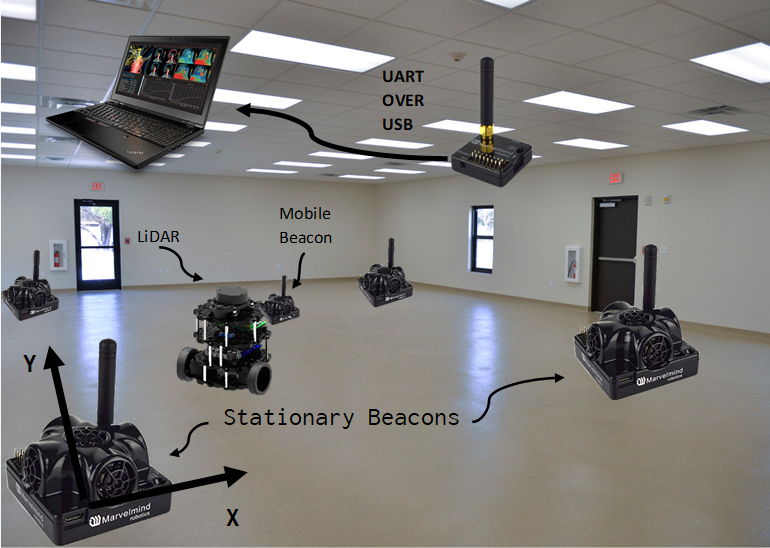
\includegraphics[width = \textwidth]{beacons.jpg}}
The final test for Dr. McCourt will involve both the Marvelmind Beacons and 
LiDAR working in conjunction with the ORPS-Robot. We will define three criteria 
to get to this point. \\
\begin{itemize}
    \item[C1.] Entry Criteria - This is where we establish that the appropriate 
    documentation, design, and requirements information is available to begin testing 
    the final system and judge correct behavior. This doesn't have to be at the very end, 
    but it must be at a stage where we can test multiple systems interacting at once.
    \item[C2.] Continuation Criteria - this defines those conditions and situations that must 
    prevail in the final testing process to allow testing to continue smoothly and robustly, that 
    serves meeting our final goal. This is also where the main stage where keeping the bug backlog 
    and having unit tests that just work without much fiddling. At this stage we want to be fighting 
    with how to use the tool, not just getting the tool to work to begin with.
    \item[C3.] Exit Criteria  - This is the criteria we must meet to determine when the project has completed 
    the main stage of testing of Dr. McCourt’s research interests. This means that no changes need to be made to 
    this completed part, except to address system test defects introduced by later stages of the project. z
\end{itemize} 
\section{Approach}

Our tests will be derived from the requirements and specifications of our project and will follow 
the following methodological approach:

\begin{itemize}
    \item[T1.] Acceptance Testing: Assess system (software \& hardware) interaction with respect 
    to user needs. For example, making sure the controller is responsive or camera is functioning 
    adequately.
    \item[T2.] System Testing: Assesses system interaction to architecture design and overall behavior. 
    For example a series of rostests that test the linking of each submodule we write for the overall 
    project.
    \item[T3.] Integration Testing: The continuous conjoining of different software artifacts to 
    serve the overall project development. For example, a test that ensures two individual modules are 
    linked properly.
    \item[T4.] Unit Testing: Assesses system interaction with respect to implementation of specific subsystems. 
    For example, a test that ensures the controller is functioning properly standalone through the joy 
    package.
\end{itemize}
While these levels are emphasized in terms of when they are applied, it is more important to distinguish 
the types of faults listed above. They are all a continuous part of the design and build process. At 
the end of the day there is an entire spectrum of testing, and much of it is hard to distinguish from 
development itself. Most tests look like unit tests and are quite simple. Other tests are more subtle, 
complex and critical. For such tests we need to use the tools laid out in this document to check our 
implementation. In the testing process the standard behavioral model should be employed, where 
execution of a program or task is represented by a behavior. A behavior is sequence of states while a state 
is an assignment of values of variables. Our program should be tested and modeled by a set of behaviors 
we define, representing possible executions. \\\\
Safety when testing can be specified using two things:\\
\begin{itemize}
    \item[-] The set of possible initial states.
    \item[-] A next-state relation, describing all possible successor states of any state. 
\end{itemize}
The above is a mindset that integrates the testing process into the development process.
\section{Fail Criteria}

\section{Testing Deliverables}

\section{Roles}

\section{Schedule}
In the testing of the different components of the final system there are always possibilities 
for unpredictable delays in the schedule, caused by either the testing or by the design. 
To stop these delays from having an effect on the overall project completion time there are a 
couple safeguards in place to ensure the project remains on schedule.\\\\
The first safeguard in place is the breaks in between quarters. In the estimation for 
completing specific tasks, the breaks between quarters was not included as optional time. 
This allows for two, 2 – 3 weeks of time, which are completely clear of other curricular 
activities, to catch up on the schedule or to get ahead.\\\\
If the breaks in between quarters is not enough time to handle the delays the first task 
besides stretch goals which will be allowed to be shortened or removed, is the testing of 
the radar sensor. The completion of the Marvel Mind positional sensors is necessary for the 
testing of Dr. McCourt’s algorithm, so the robot’s primary purpose will still be able to 
function without a completely tested radar system.\\\\
Testing the controller and robot movement functionality is scheduled for the first two weeks 
after the completion of getting the controller and the robot running. The current predicted date 
for those two weeks is Jan $7^{th}$ to Jan $21^{st}$.\\\\\
The testing of the Marvel Mind positional sensors is scheduled for the first 4 weeks after the 
completion of the installation of both the Marvel Mind sensors and the radar sensor. This time 
segment is currently supposed to be April $1^{st}$ to April $28^{th}$.\\\\
The testing of the radar sensor will be concurrent with the testing of the Marvel Mind sensors, 
however the marvel Mind sensors will take priority. If due to any past delays, the sensor testing 
is not completed by the time the algorithm testing should start, the testing will move on to that 
of the algorithm, and the radar testing will be fit in if there is any extra time.\\\\
On completion of the Marvel Mind sensors testing, we will be able to test our implementation 
Dr. McCourt’s algorithm. This is scheduled for the 4 weeks after the completion of the Marvel 
Mind sensor testing. The current expected dates are April $28^{th}$ to March $26^{th}$.\\\\
If all the previous tasks are completed before March $26^{th}$, we will attempt to complete the image 
recognition stretch goal. At this point there would only be this optional task at hand, so the 
testing would last as long as it could before project presentation day. The decision of showcasing 
this feature will depend on how well it is running by that day.
\section{Testing Risks and Mitigation}

\section{Approvals}

\end{document}